\documentclass[../main.tex]{subfiles}
\begin{document}

\section{Optimal Control of Pitch/Travel with Feedback (LQ)}
In this task we add feedback to the optimal controller that we developed in \cref{kap:Part2OptimalControlWithoutFeedback}.

\subsection{Motivation}
The experimental results in \cref{kap:task_10_2_experimental_results} clearly shows that planning a sequence of inputs does not produce the expected sequence of outputs - as that section explains there are many reasons for travel-drift. In situations with drift without feedback then the output will not follow the planned trajectory, but adding feedback could compensate for the drift and offset and therefore reduce or eliminate the deviation from the planned trajectory.

The results achieved in this section shows that adding feedback greatly improves performance.

\subsection{Introducing feedback}
There are many approaches to adding feedback, but in this assignment only two will be considered: linear state feedback and model predictive control.

\textbf{Linear state feedback} adds a new control layer below the optimization layer, the advanced control layer. This layer controls the pitch setpoint to the basic control layer based on a control law that considers the optimal trajectory and the current state of the system\todo{Er det mulig å dele opp setningen noe?}. If the states deviate from the optimal value the input is changed according to the pitch-control equation:
\begin{equation}\label{eq:lab3_feedback}
	u_k = u_k^* - \bm{K}^T(\bm x_k - \bm x_k^*)
\end{equation}
where $u_k^*$ and $\bm x_k^*$ are the optimal input and state trajectories predicted in the optimization layer, $u_k$ is the next input and $x_k$ is the current state. $K$ is the linear state feedback gain. 

In this exercise the gain matrix $K$ is calculated as an infinite horizon LQ controller, see \cref{kap:task_10_3_LQ_controller} for more info about the exact implementation.

\textbf{Model Predictive Control (MPC)} is a completely different solution: the optimal trajectory is recalculated at every timestep - instead of compensating for deviation from optimal, the optimal is recalculated to get a new possible trajectory based on the current states. See \cref{kap:10_3_mpc} for more info about how that could be implemented here.

\subsection{LQ controller} \label{kap:task_10_3_LQ_controller}
A Linear Quadratic (LQ) controller minimizes the quadratic objective function:
\begin{equation}
    J = \sum^\infty_{i=0} \Delta x_{i+1}^\top Q \Delta x_{i+1} + \Delta u_i^\top R \Delta u_i, \quad Q \ge0, \quad R > 0
\end{equation}
for a linear model
\begin{equation}\label{eq:lab3_lin_model}
	\Delta x=A\Delta x_i + B \Delta u_i
\end{equation}
Here $ \Delta x = x - x^*$ and $\Delta u = u - u^*$ are deviations from the optimal trajectory.

This formulation is an infinite horizon linear quadratic regulator which has a solution with a constant linear feedback gain, $K$ - which is exactly what was specified previously! Note that this regulator does not have any constraints.

\subsubsection{Choosing the weights}
The matrix $Q$ and the scalar $R$ are the weights of the optimalization problem. $Q$ determines how much state-deviations should be penalized, while $R$ determines how much input-deviation should be punished\todo{``penalized'' her og siden du bruker det om Q? Eller blir det rart?}. What needs to prioritized depends on the application.

In this case the system is a helicopter where the goal is to control the travel of the helicopter. The travel is the most important state, while travelrate, pitch and pitchrate are secondary. Thus it makes sense to prioritize keeping travel close to the planned trajectory - it is of course not possible to keep all states close to the trajectory. This motivates a \textbf{state-weight} with relatively high value related to travel.\todo{Meget bra skrevet!}

The input from the LQR regulator is the pitch-setpoint - which in this case does not need to follow the planned optimal trajectory. Thus a low \textbf{input-weight} is warranted\todo[inline]{Kan du si noe om hvorfor? Bare nevne at lavere R gir høyere input og motsatt. Så du skrev om penalize over, men kanskje vi skal forklare at høyere verdier straffer mer? Eller er det overflødig?}. \textit{However} the pitch-setpoint has a constraint but this implementation of LQR does not have any constraints! The result is that input-use could fall outside the constraint imposed on the optimization layer (this is clearly happening in the experiments performed in the lab) \todo{Hvor skjer dette i laben? Mulig å referere til figur? Og hvordan ser man at dette skjer?}.

\subsubsection{Calculating the solution}
Calculating the solution to the LQR problem is trivial using Matlab:
\begin{lstlisting}[language=Matlab]
% The discrete system described as a state space system, Ad and Bd must be defined

% W1 is the weigth of travel
% W2 is the weight of travelrate
% W3 is the weight of pitch
% W4 is the weight of pitchrate
Q = diag([W1, W2, W3, W4]);

% W5 is the weight of the input
R = W5;

% The function dlqr is used to solve the LQR problem
[K, S, e] = dlqr(Ad, Bd, Q, R);
\end{lstlisting}

\subsection{Model Predictive Control}\label{kap:10_3_mpc}
Model Predictive Control is another way of introducing feedback to an optimal control system. In an MPC controlled system the optimal response and input is recalculated at every timestep, the input used is simply the first of the optimal input values calculated at every step.

This is a drastically different approach to the LQ-method impemented in this laboratory exercise.

\subsubsection{Modified Control Hierarchy with MPC}
Rather than introducing the Advanced Control Layer with the LQ-controller, introducing MPC would introduce the feedback to the Optimization Layer instead.\todo{Bra forklaring!! Hvis dette med en modifisert figur?} The optimization layer would use the current state value and generate an optimal trajectory to the target, outputting pitch-setpoints to the Basic control layer at every timestep.

\todo[inline]{Denne seksjonen svarer bare på en tredjedel av det spørsmålet spør om:


``How would you realize this controller? Discuss advantages and disadvantages with an MPC controller compared to the controller you have implemented. Also, How would the structure in Figure 8 look like if you used MPC.
''


Her mangler man altså den biten om fordeler/ulemper, samt et bilde av hvordan MPC blir implementert.
}

\subsection{Experimental results}\label{sec:lab3_result}
The group performed a host of controlled tests with different tunings within five different targets:
\begin{enumerate}
	\item Prioritizing input use, see \cref{fig:LAB3_R_variations}
	\item Prioritizing travel, see \cref{fig:LAB3_Q_variations_travel}
	\item Prioritizing travelrate, see \cref{fig:LAB3_Q_variations_travelrate}
	\item Prioritizing pitch, see \cref{fig:LAB3_Q_variations_pitch}
	\item Prioritizing pitchrate, see \cref{fig:LAB3_Q_variations_pitchrate}
\end{enumerate}

It is very clear that introducing feedback produced results much better than the ones achieved without feedback, almost regardless of the tuning of the LQR regulator.

Prioritizing input usage only has a slight effect, the input usage does get slightly closer to the planned trajectory but not by much. This could be pushed further by weighing states lower, but this was not explored as doing so will only result in the same system as the previous lab-exercise where u was exactly the planned trajectory.\todo[inline]{Kult poeng, kan du forklare hvorfor? Jeg skjønner det ikke...} Interestingly the \textit{pitch-response}, a state, is improved because of the close relation to the setpoint. \todo [inline]{Setpoint til hva? Kanskje fjerne ``a state''; det burde man jo skjønne ut fra pitch-response?}

Prioritizing travel has a great effect on the travel response - resulting in almost perfect travel response. Unfortunately this also introduced oscillations in pitch-setpoint, pitch and pitchrate.
\todo[inline]{Blir det oscillering i pitch setpoint også? Det vises vell ikke i plottene?}

Prioritizing travelrate, pitch and pitchrate results in responses closer to the planned trajectory\todo[inline]{Til korresponderende traj., eller travel traj?}, but this is not further discussed as travel is the state most important to control - theese experiments were only to show that it would be possble should another state be valuable.

\subsubsection{Possible improvements}
The group observed that the state never reached the optimal trajectory, even with very high Q-values. The group believes that adding integration to the LQ-regulator would eliminate the stationary offset between travel and the planned travel trajectory. 

Another improvement is to impose a constraint on the input-use on the advanced control layer to respect the maximum pitch-setpoint stipulated in the problem description.\todo[inline]{Komplisert setning, jeg sliter med å forstå hva den betyr...} This could either be achieved using a different feedback strategy, or by simply saturating the input. If the simple limiting saturation is chosen then it would make sense to set the optimizatoin layers constraint slightly lower to limit the saturation.

\todo[inline]{Kan det være lurt å nevne at vi også kan endre q i cost function slik vi får en mer realiserbar optimal trajectory?}

\subsubsection{Plots}

\begin{figure}[h]
	\centering
    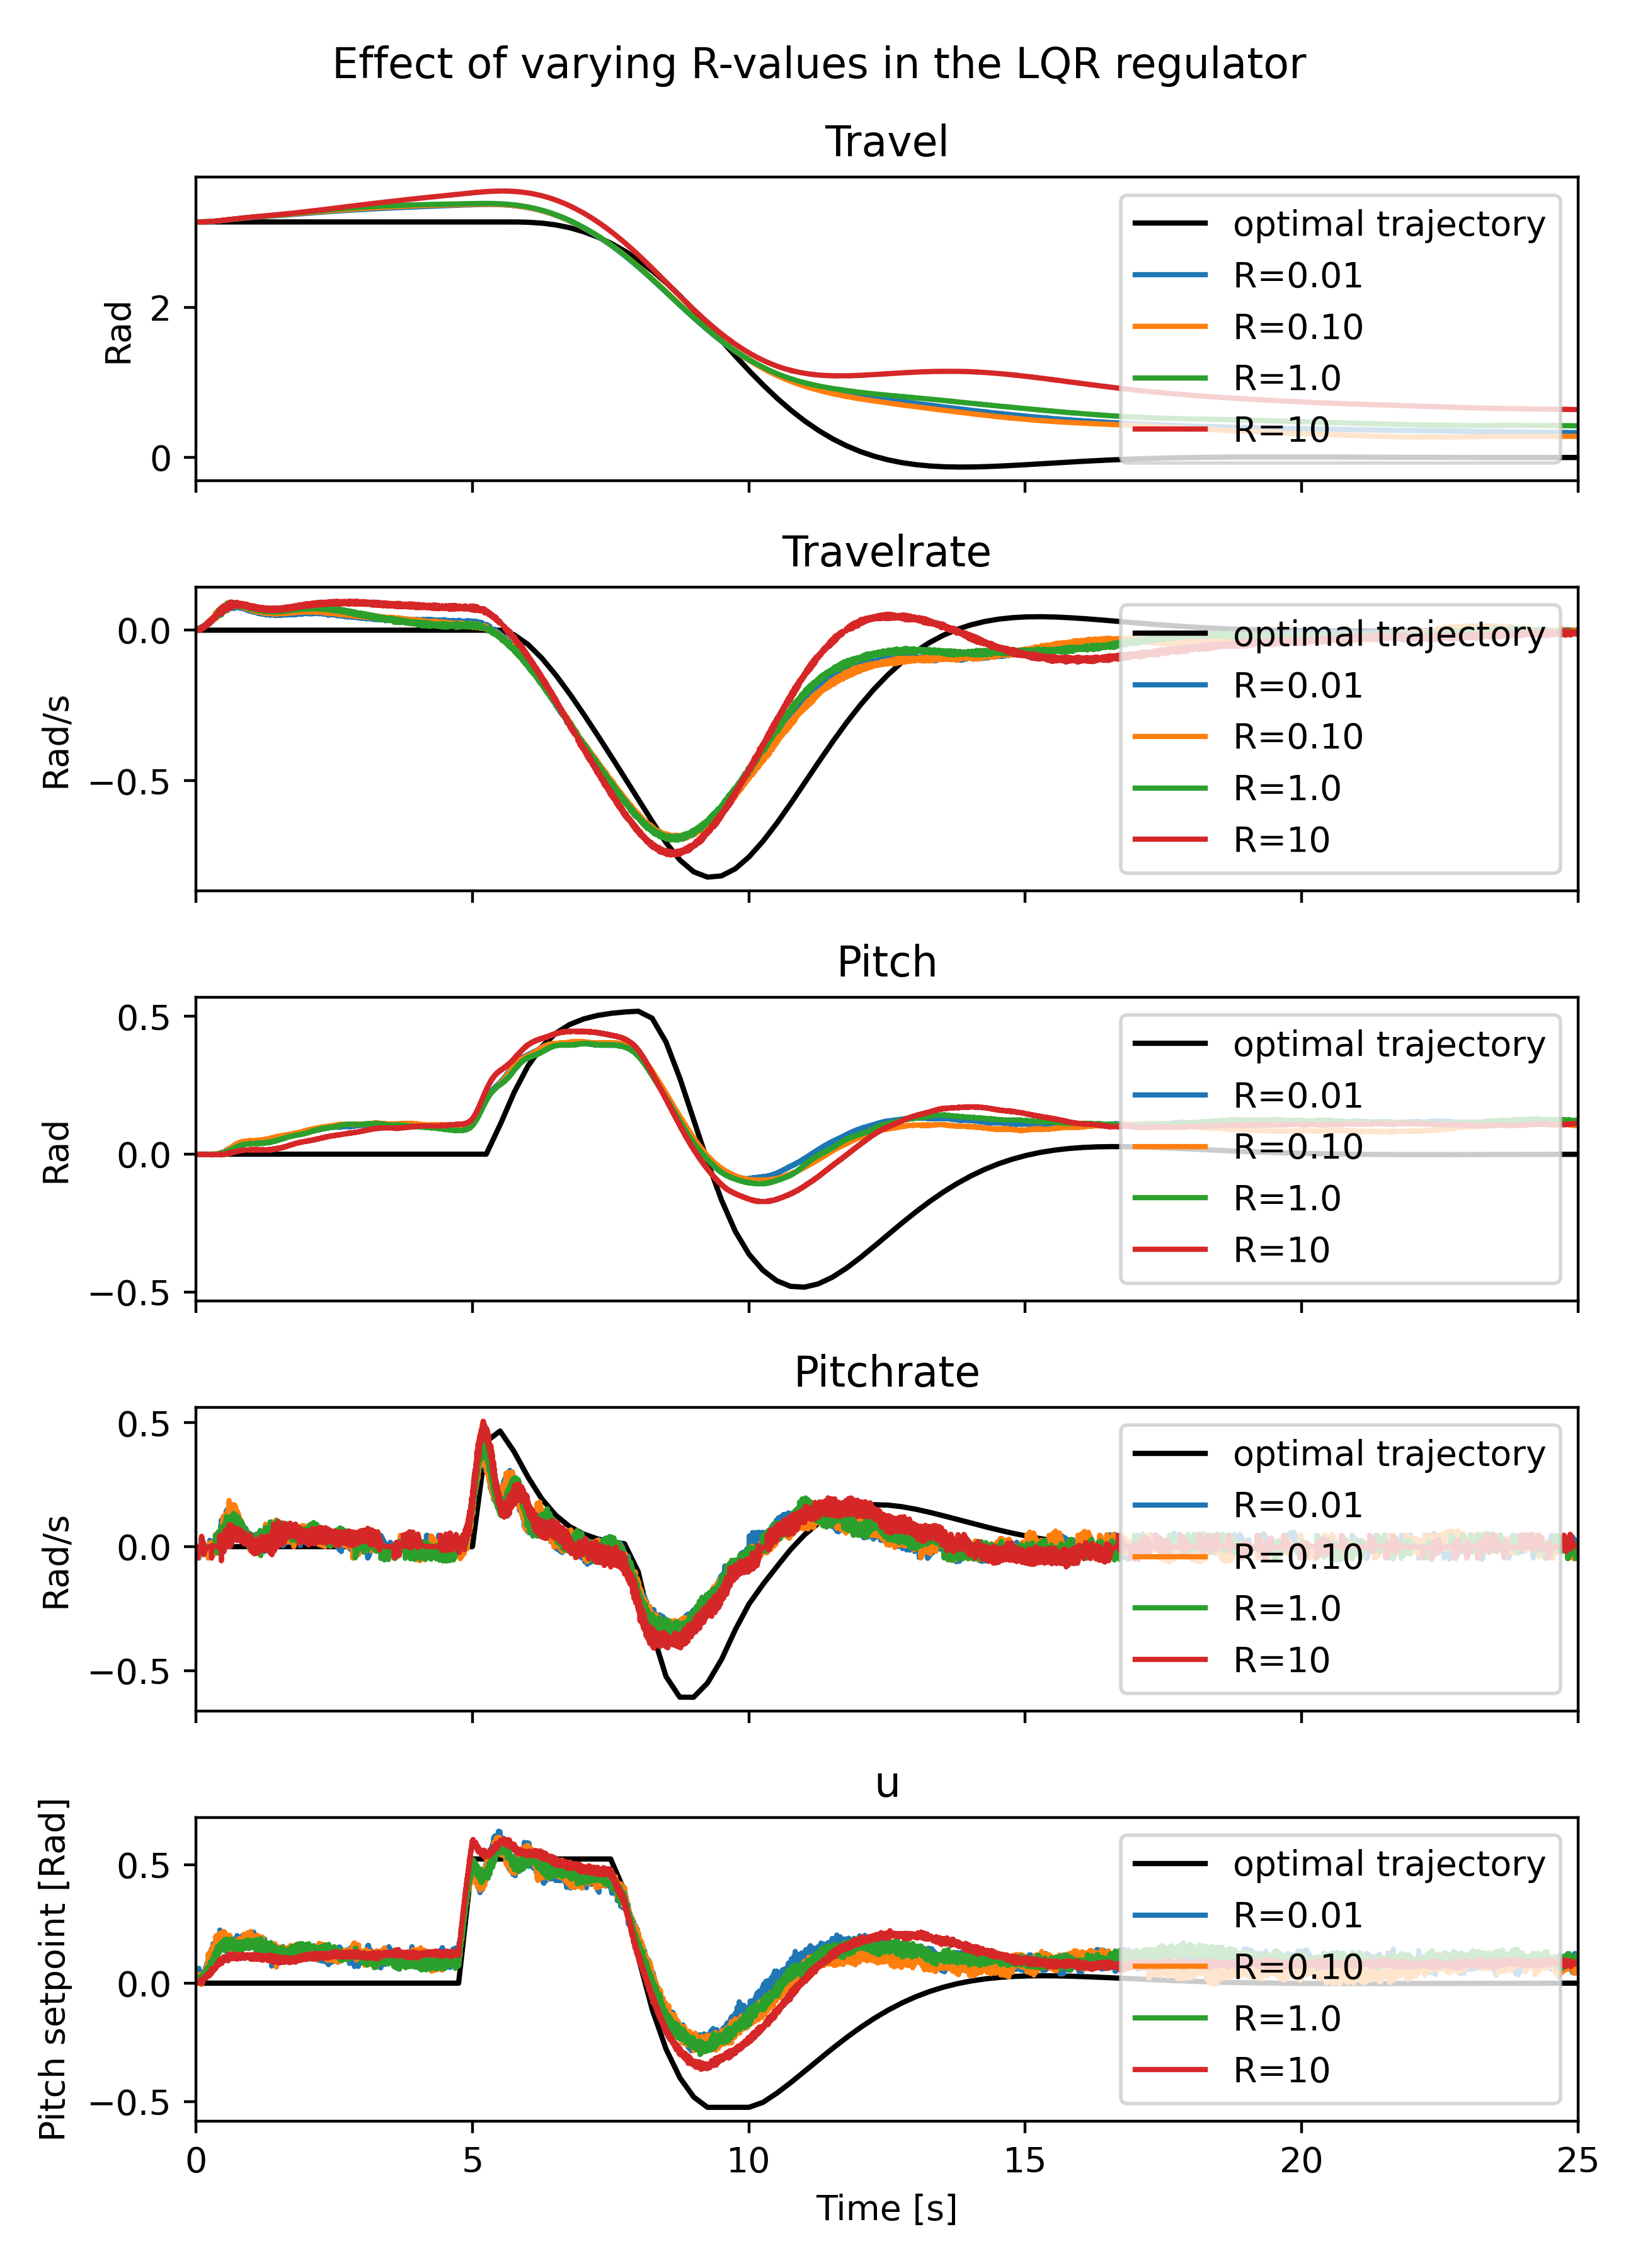
\includegraphics[width=0.8\linewidth]{figures/LAB3_R_variations.png}
	\caption{Prioritizing input-usage while keeping Q=diag([1,1,1,1]). This shows a very slight difference between weights. No further experimentation was done because if $u_k = u_k^*$ then that would be the same as the previous exercise.}
	\label{fig:LAB3_R_variations}
\end{figure}

\begin{figure}[h]
	\centering
	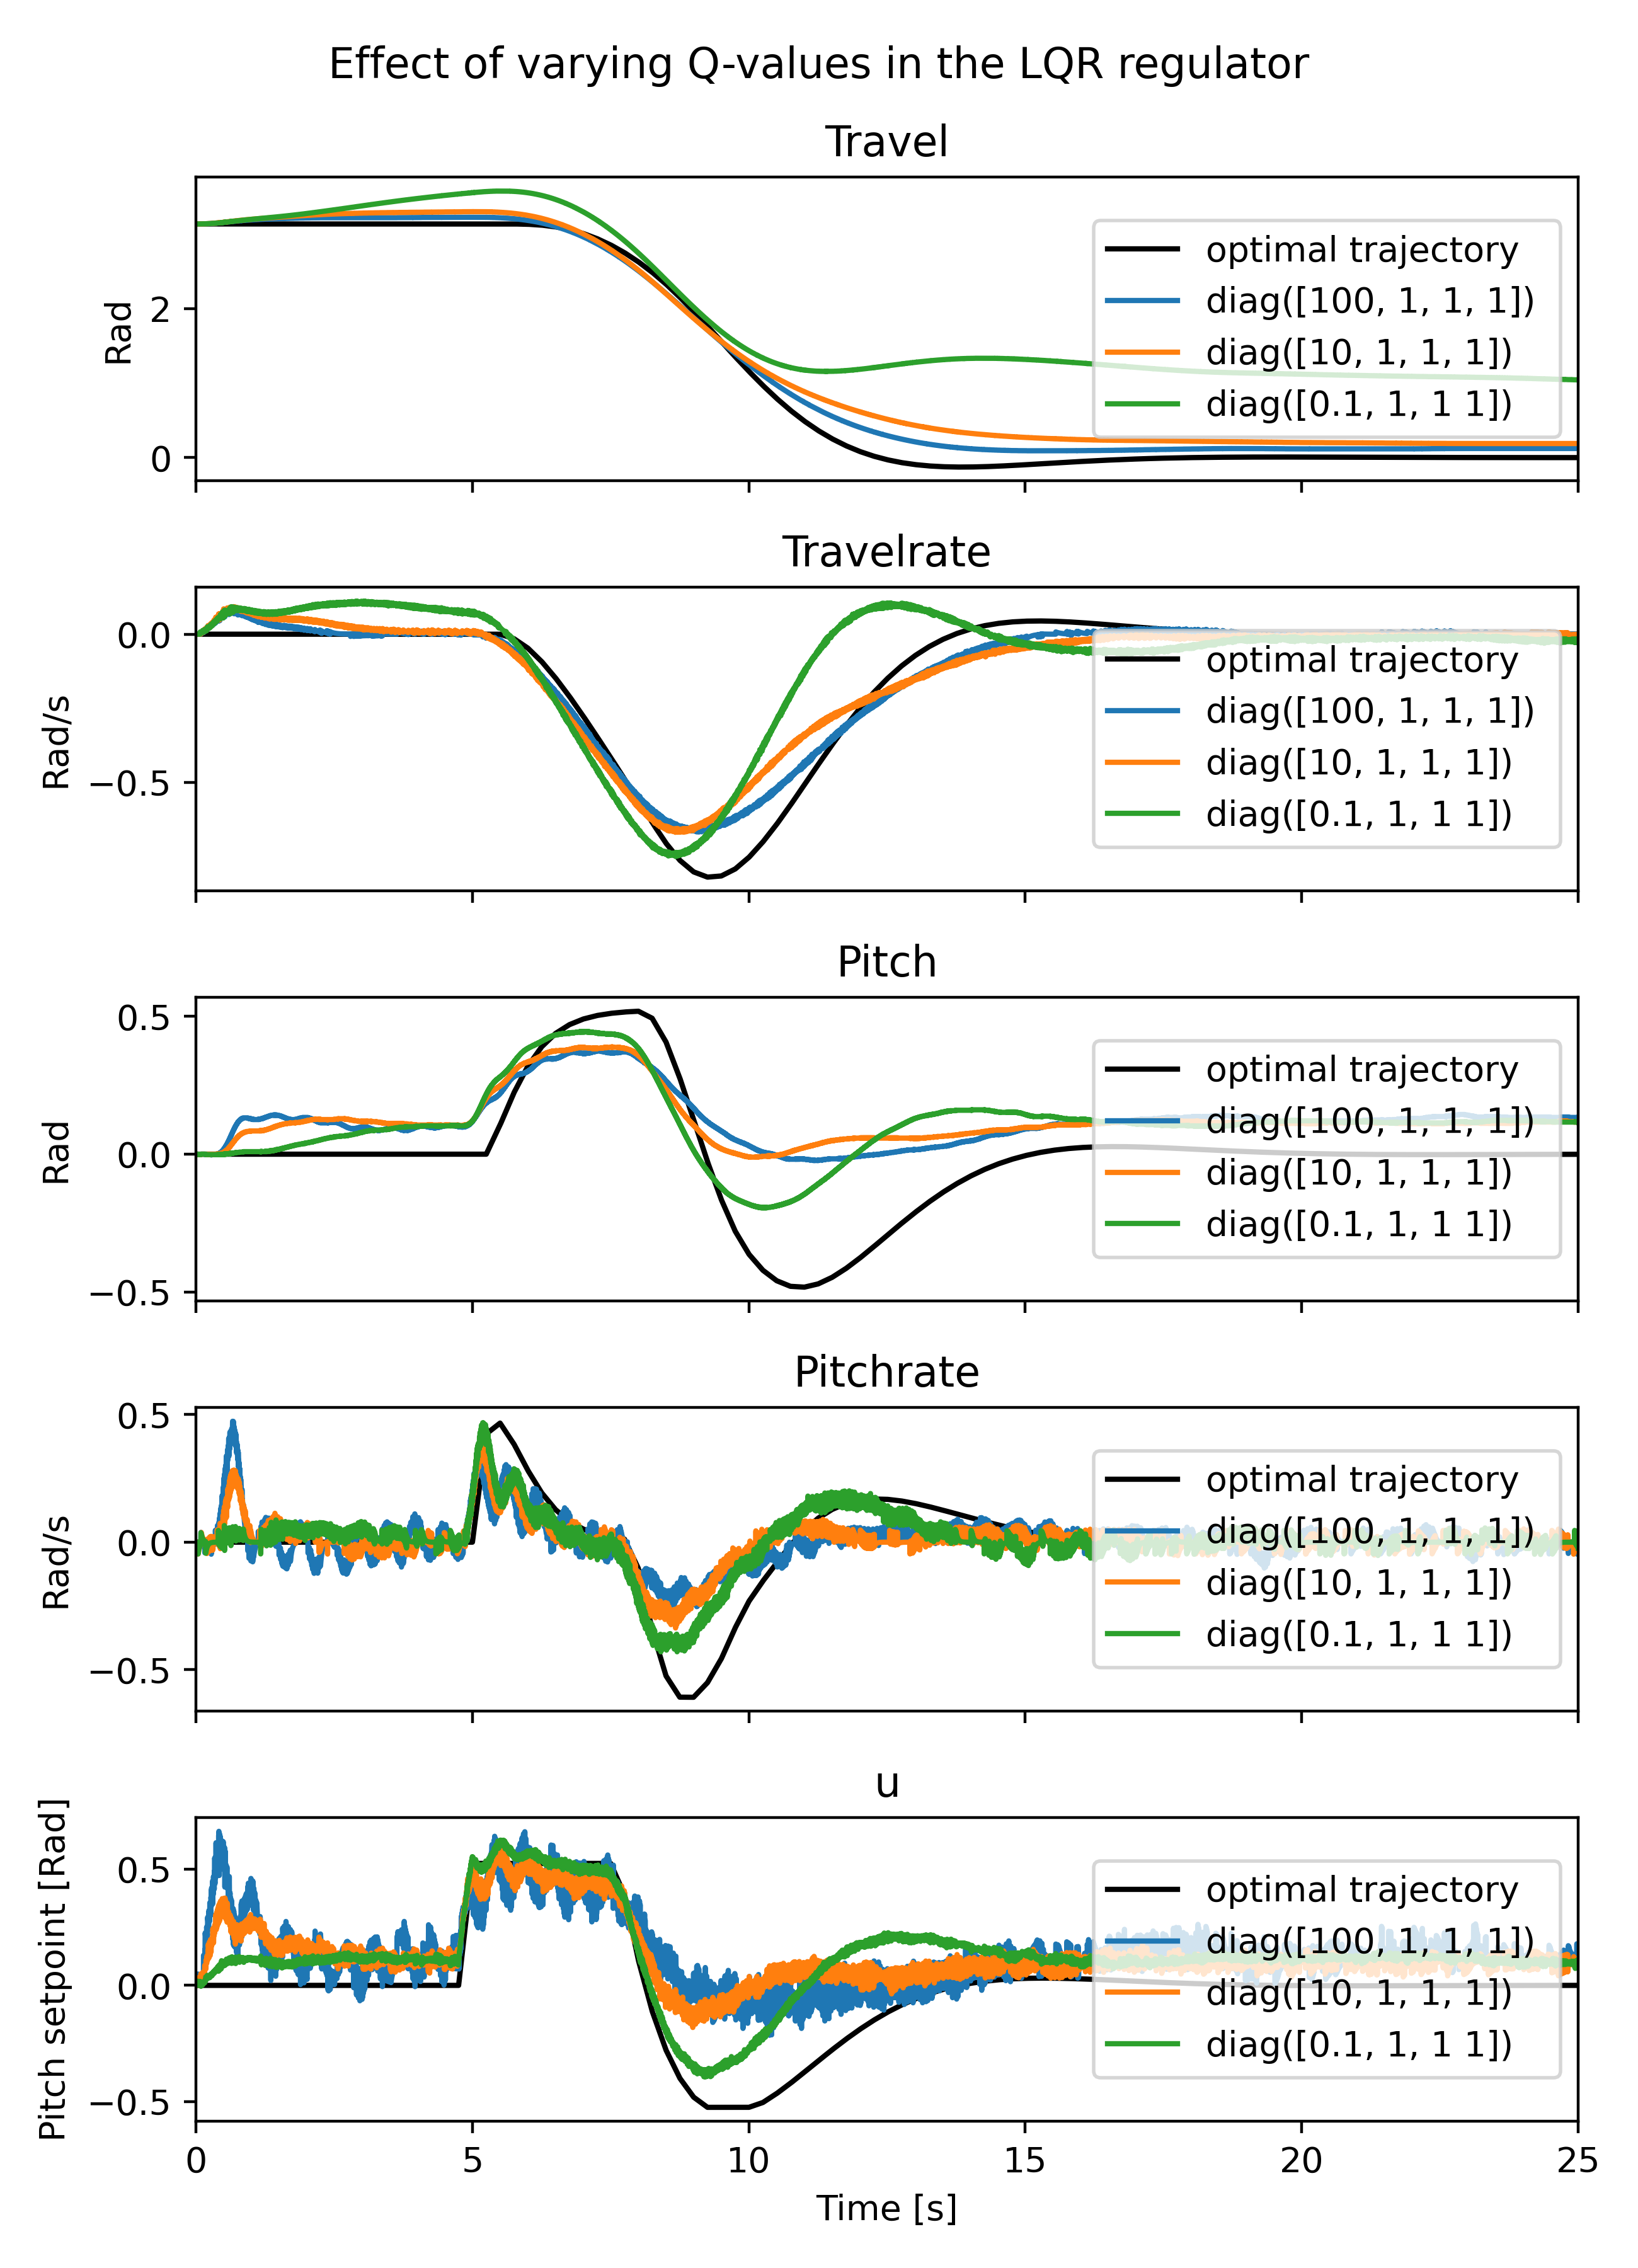
\includegraphics[width=0.8\linewidth]{figures/LAB3_Q_variations.png}
	\caption{Prioritizing the weight related to travel while keeping $R=1$. This was very effective in reducing offset between travel and the planned trajectory. Unfortunately at heigher gains there is some offset introducted and even then there is still a constant offset. A regulator with integral action would probably eliminate this offset without introducting oscillations.}
	\label{fig:LAB3_Q_variations_travel}
\end{figure}

\begin{figure}[h]
	\centering
	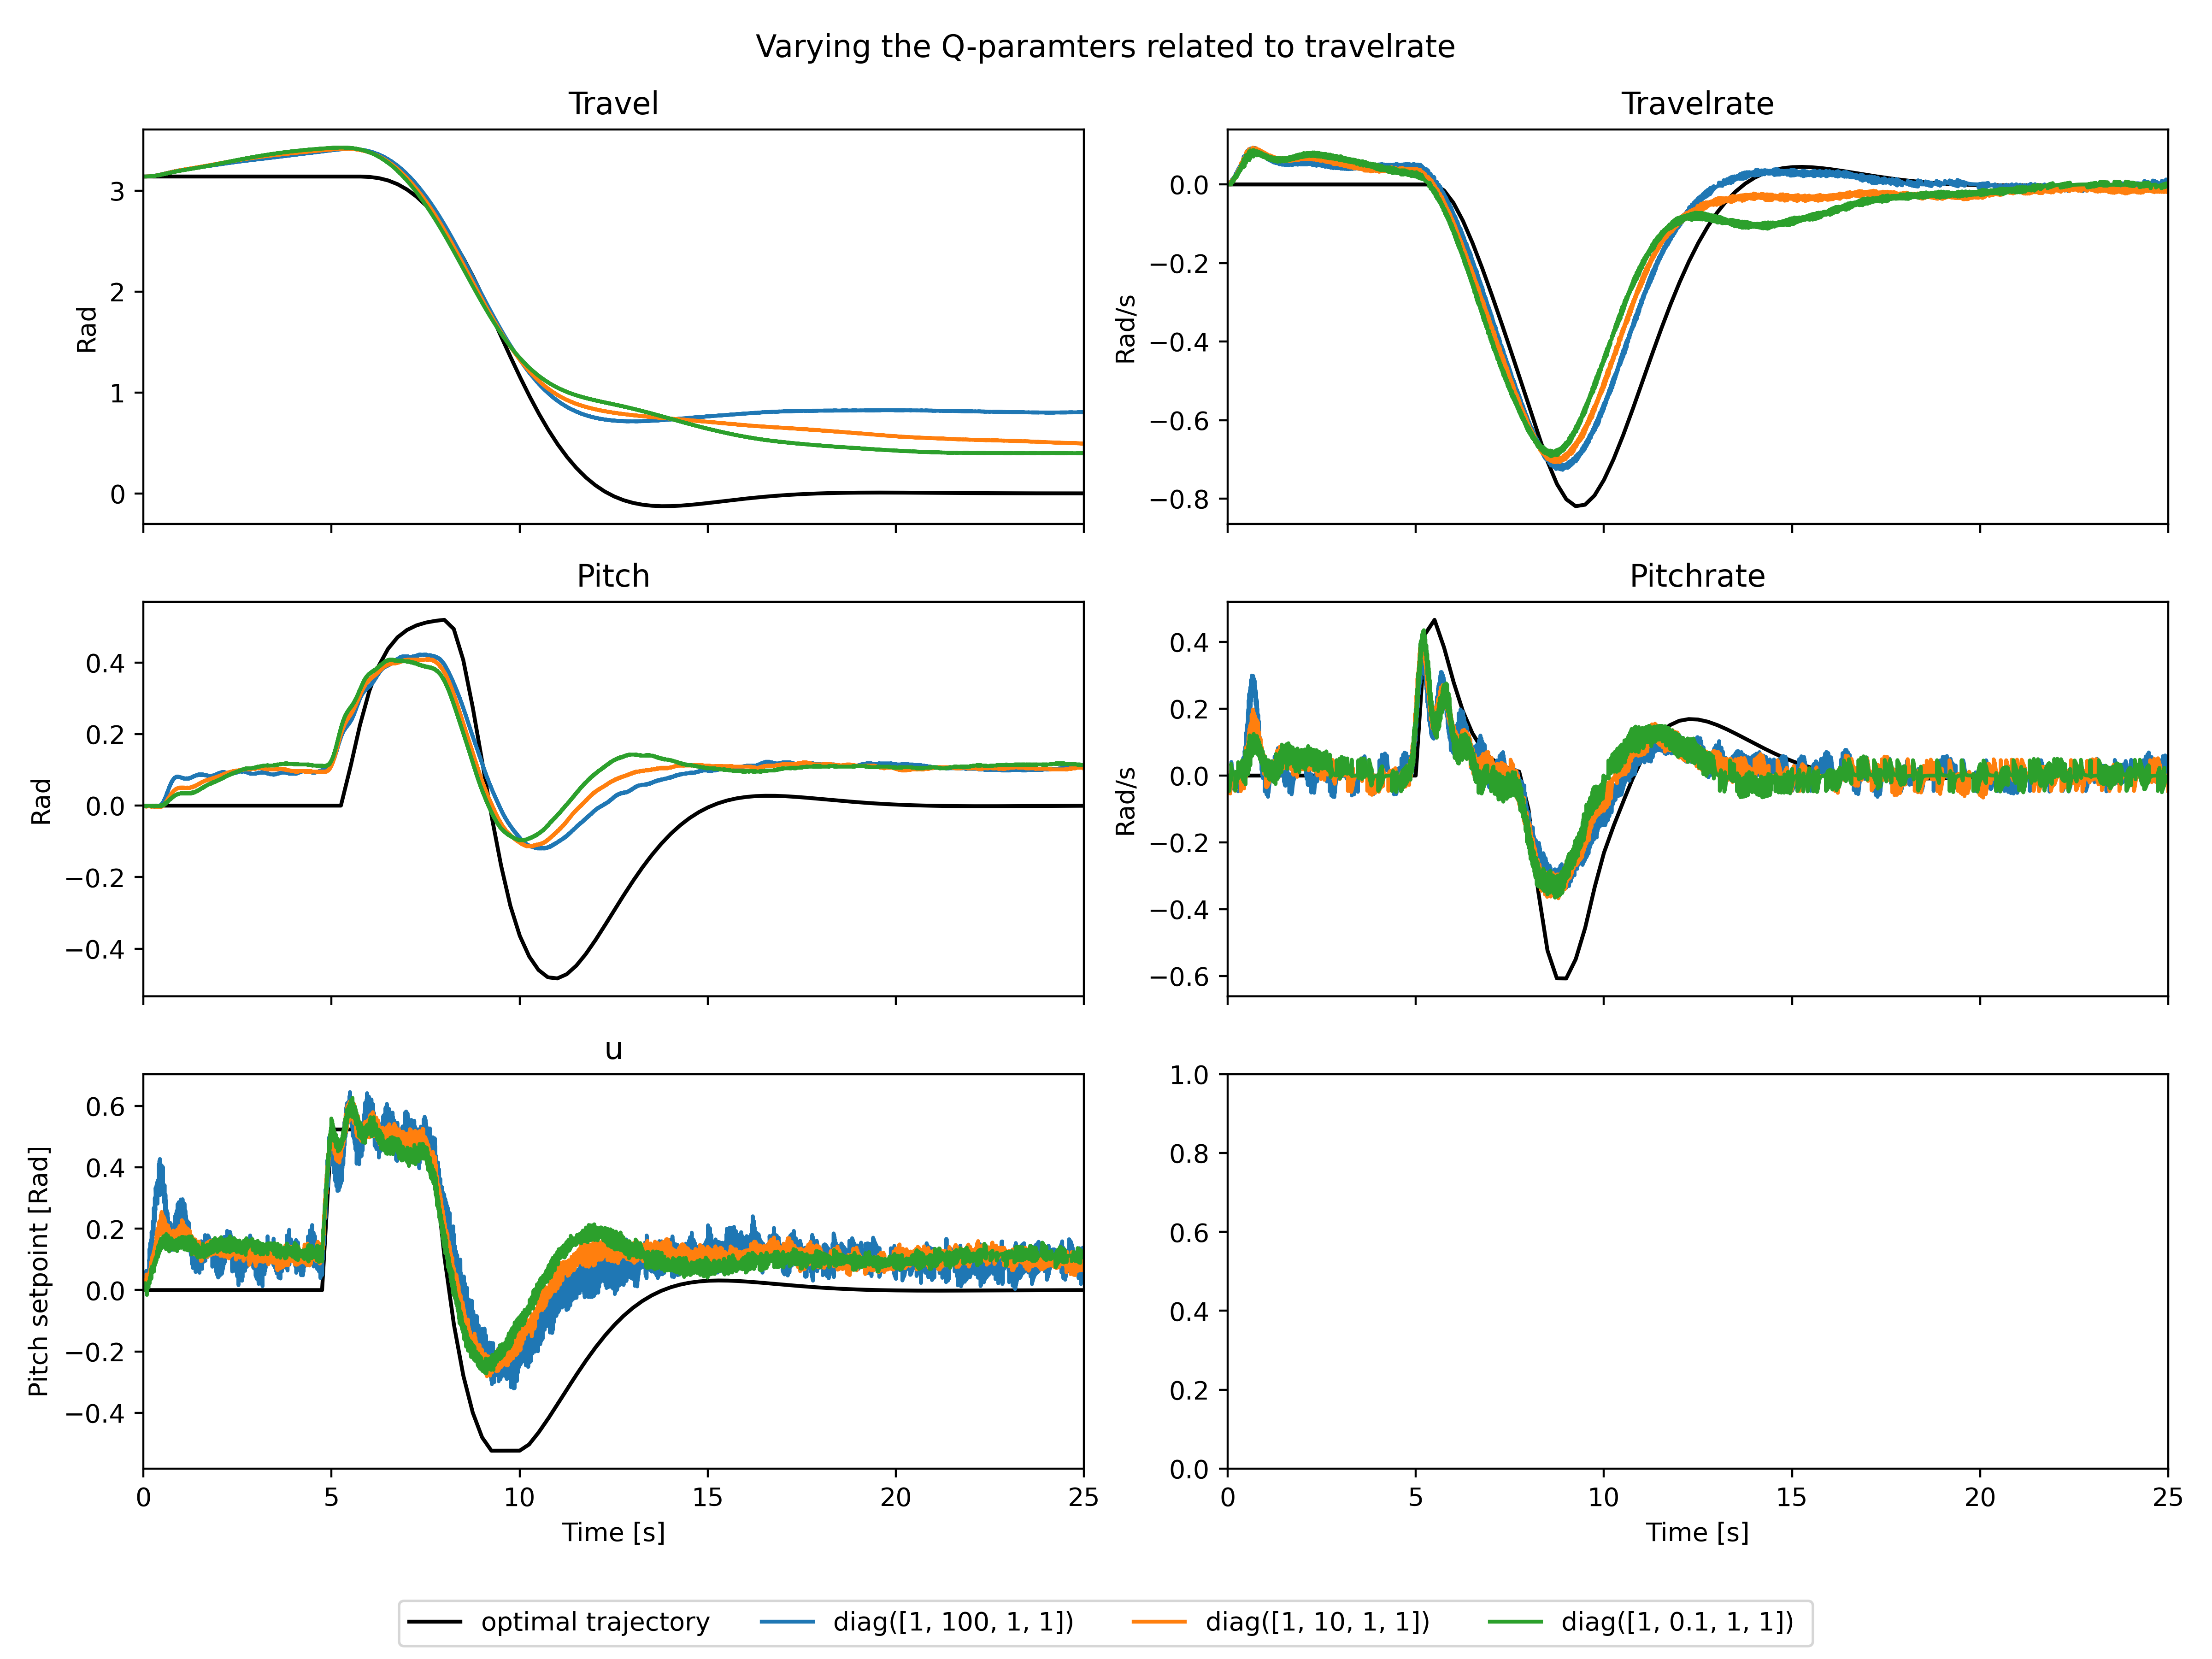
\includegraphics[width=0.8\linewidth]{figures/LAB3_Q_variations_travelrate.png}
	\caption{Changing the weight of the travelrate state, $R=1$. This had only a minor effect with small variations in the response.}
	\label{fig:LAB3_Q_variations_travelrate}
\end{figure}

\begin{figure}[h]
	\centering
	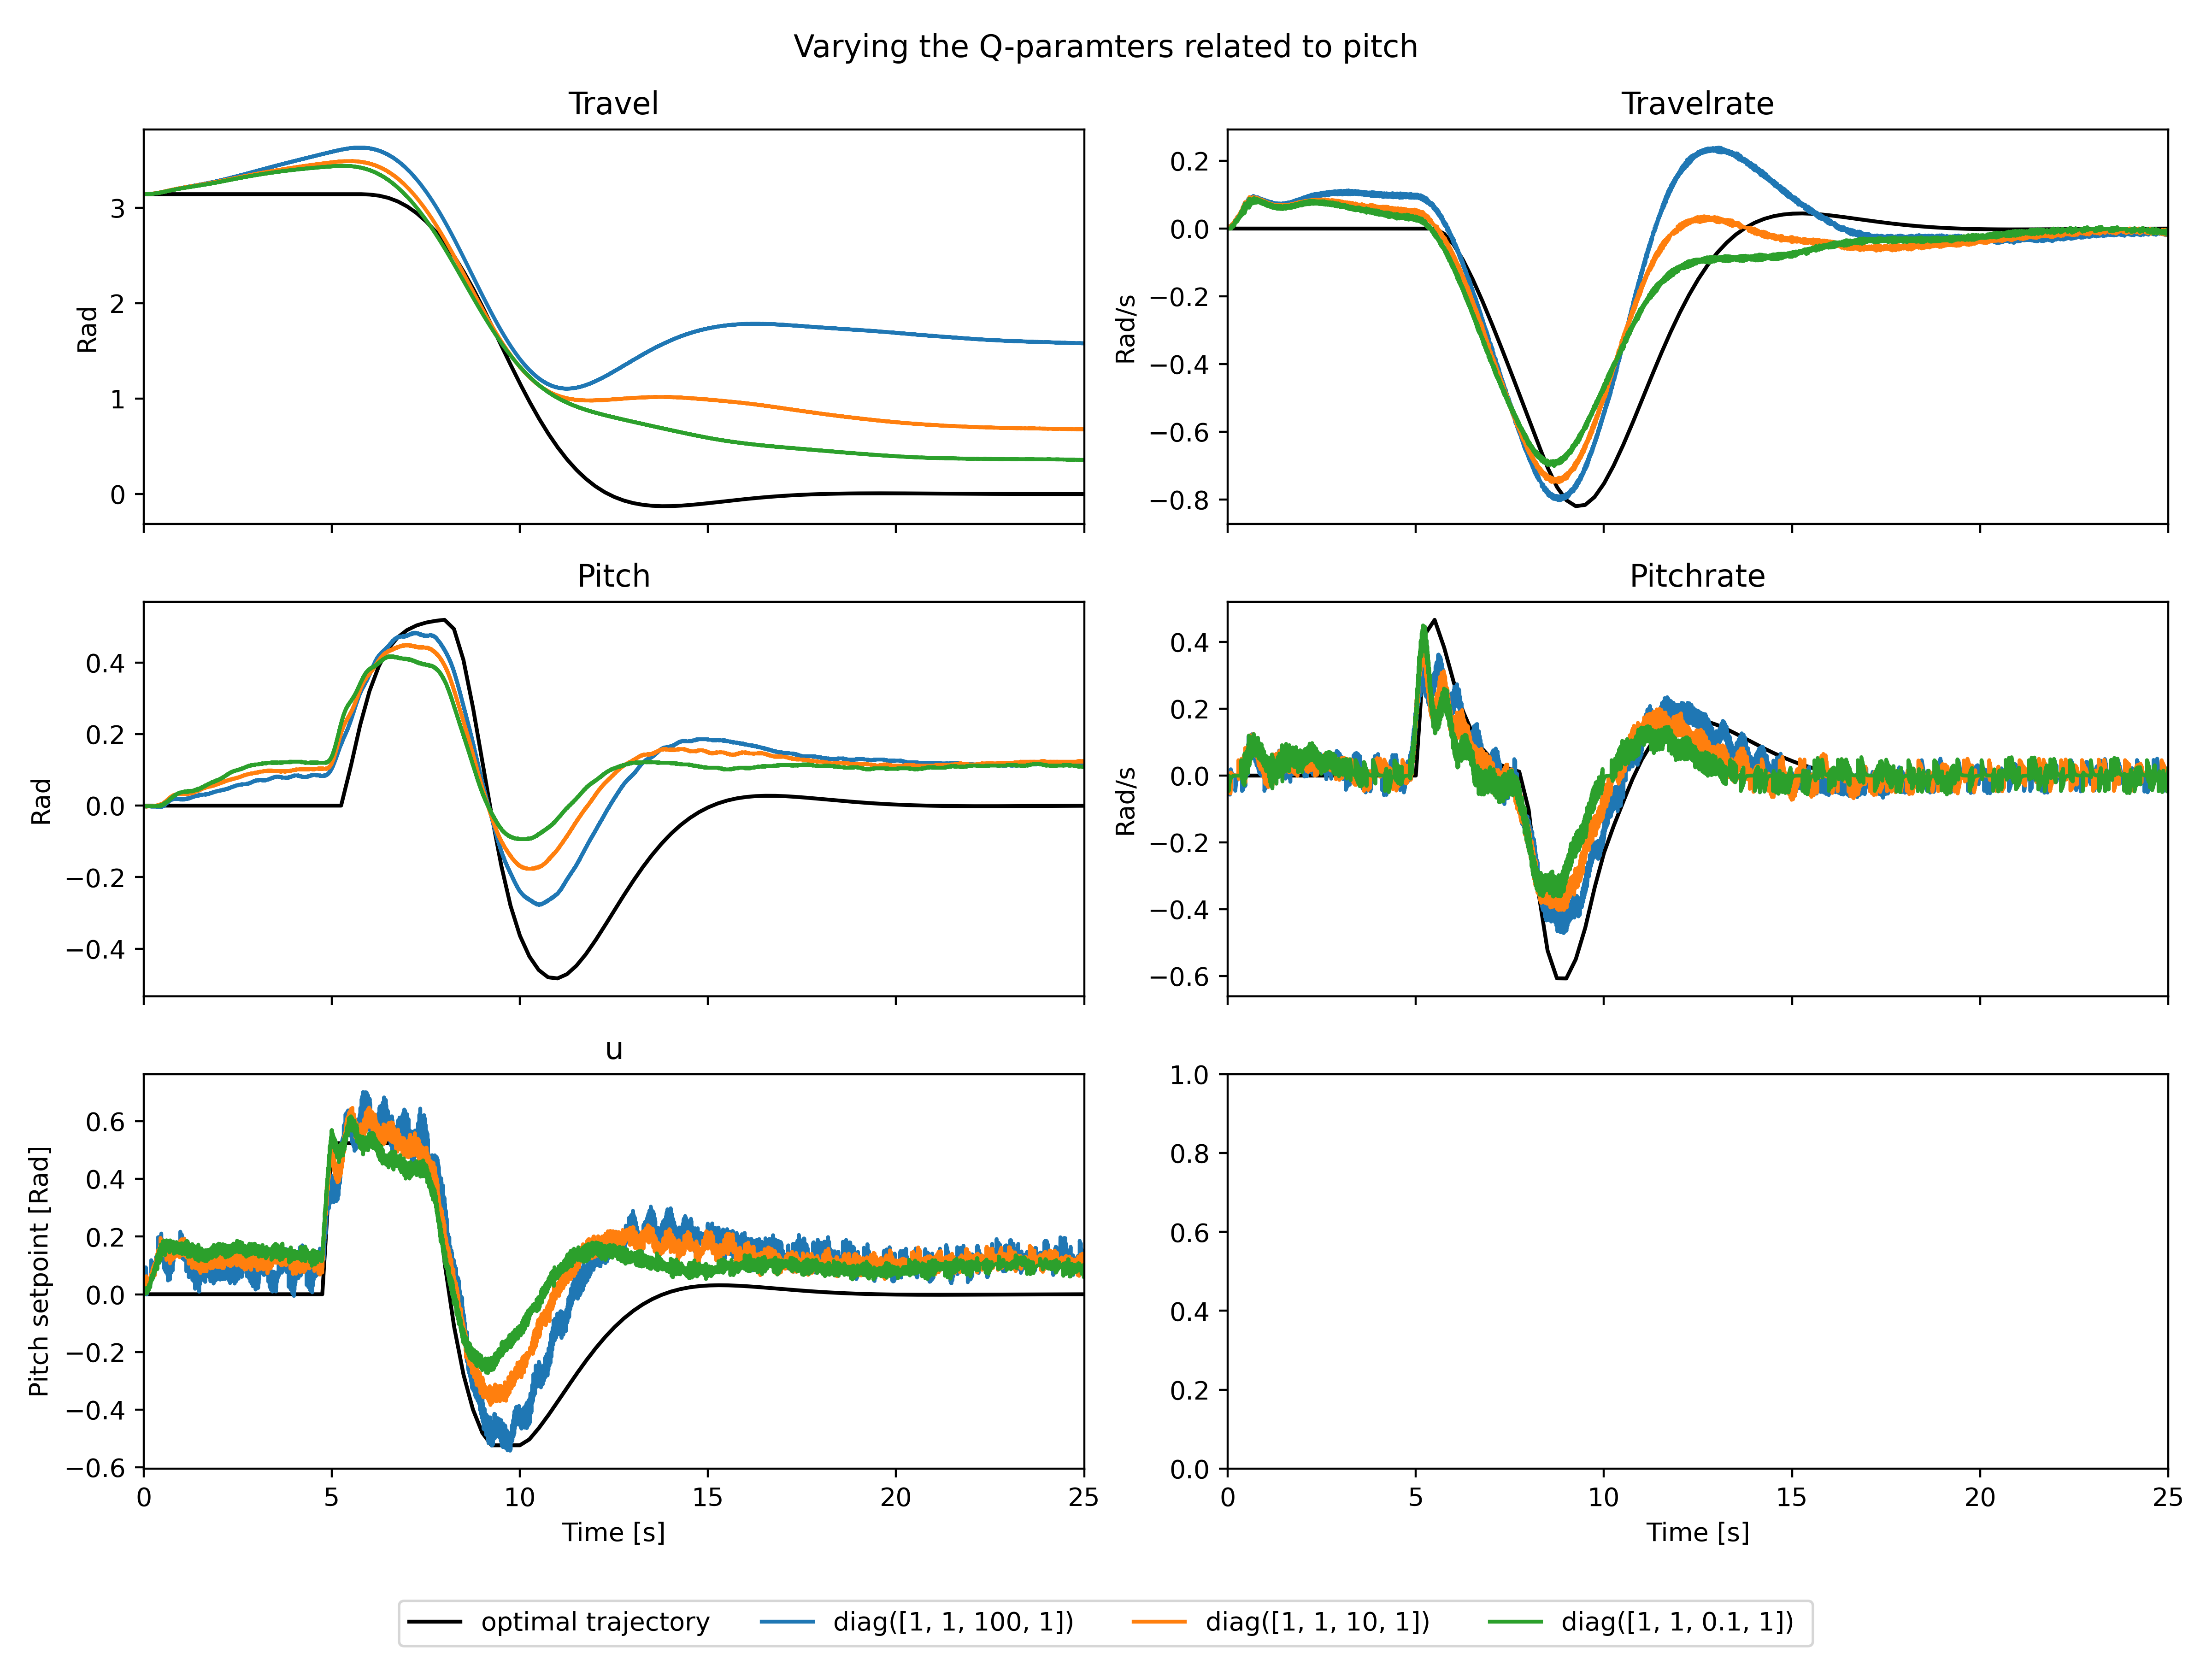
\includegraphics[width=0.8\linewidth]{figures/LAB3_Q_variations_pitch.png}
	\caption{Changing the weight of the pitch state, $R=1$. This had the effect of getting both pitch, pitch-setpoint and pitchrate closer to the planned trajectory at the expense of travel and travelrate.}
	\label{fig:LAB3_Q_variations_pitch}
\end{figure}

\begin{figure}[h]
	\centering
	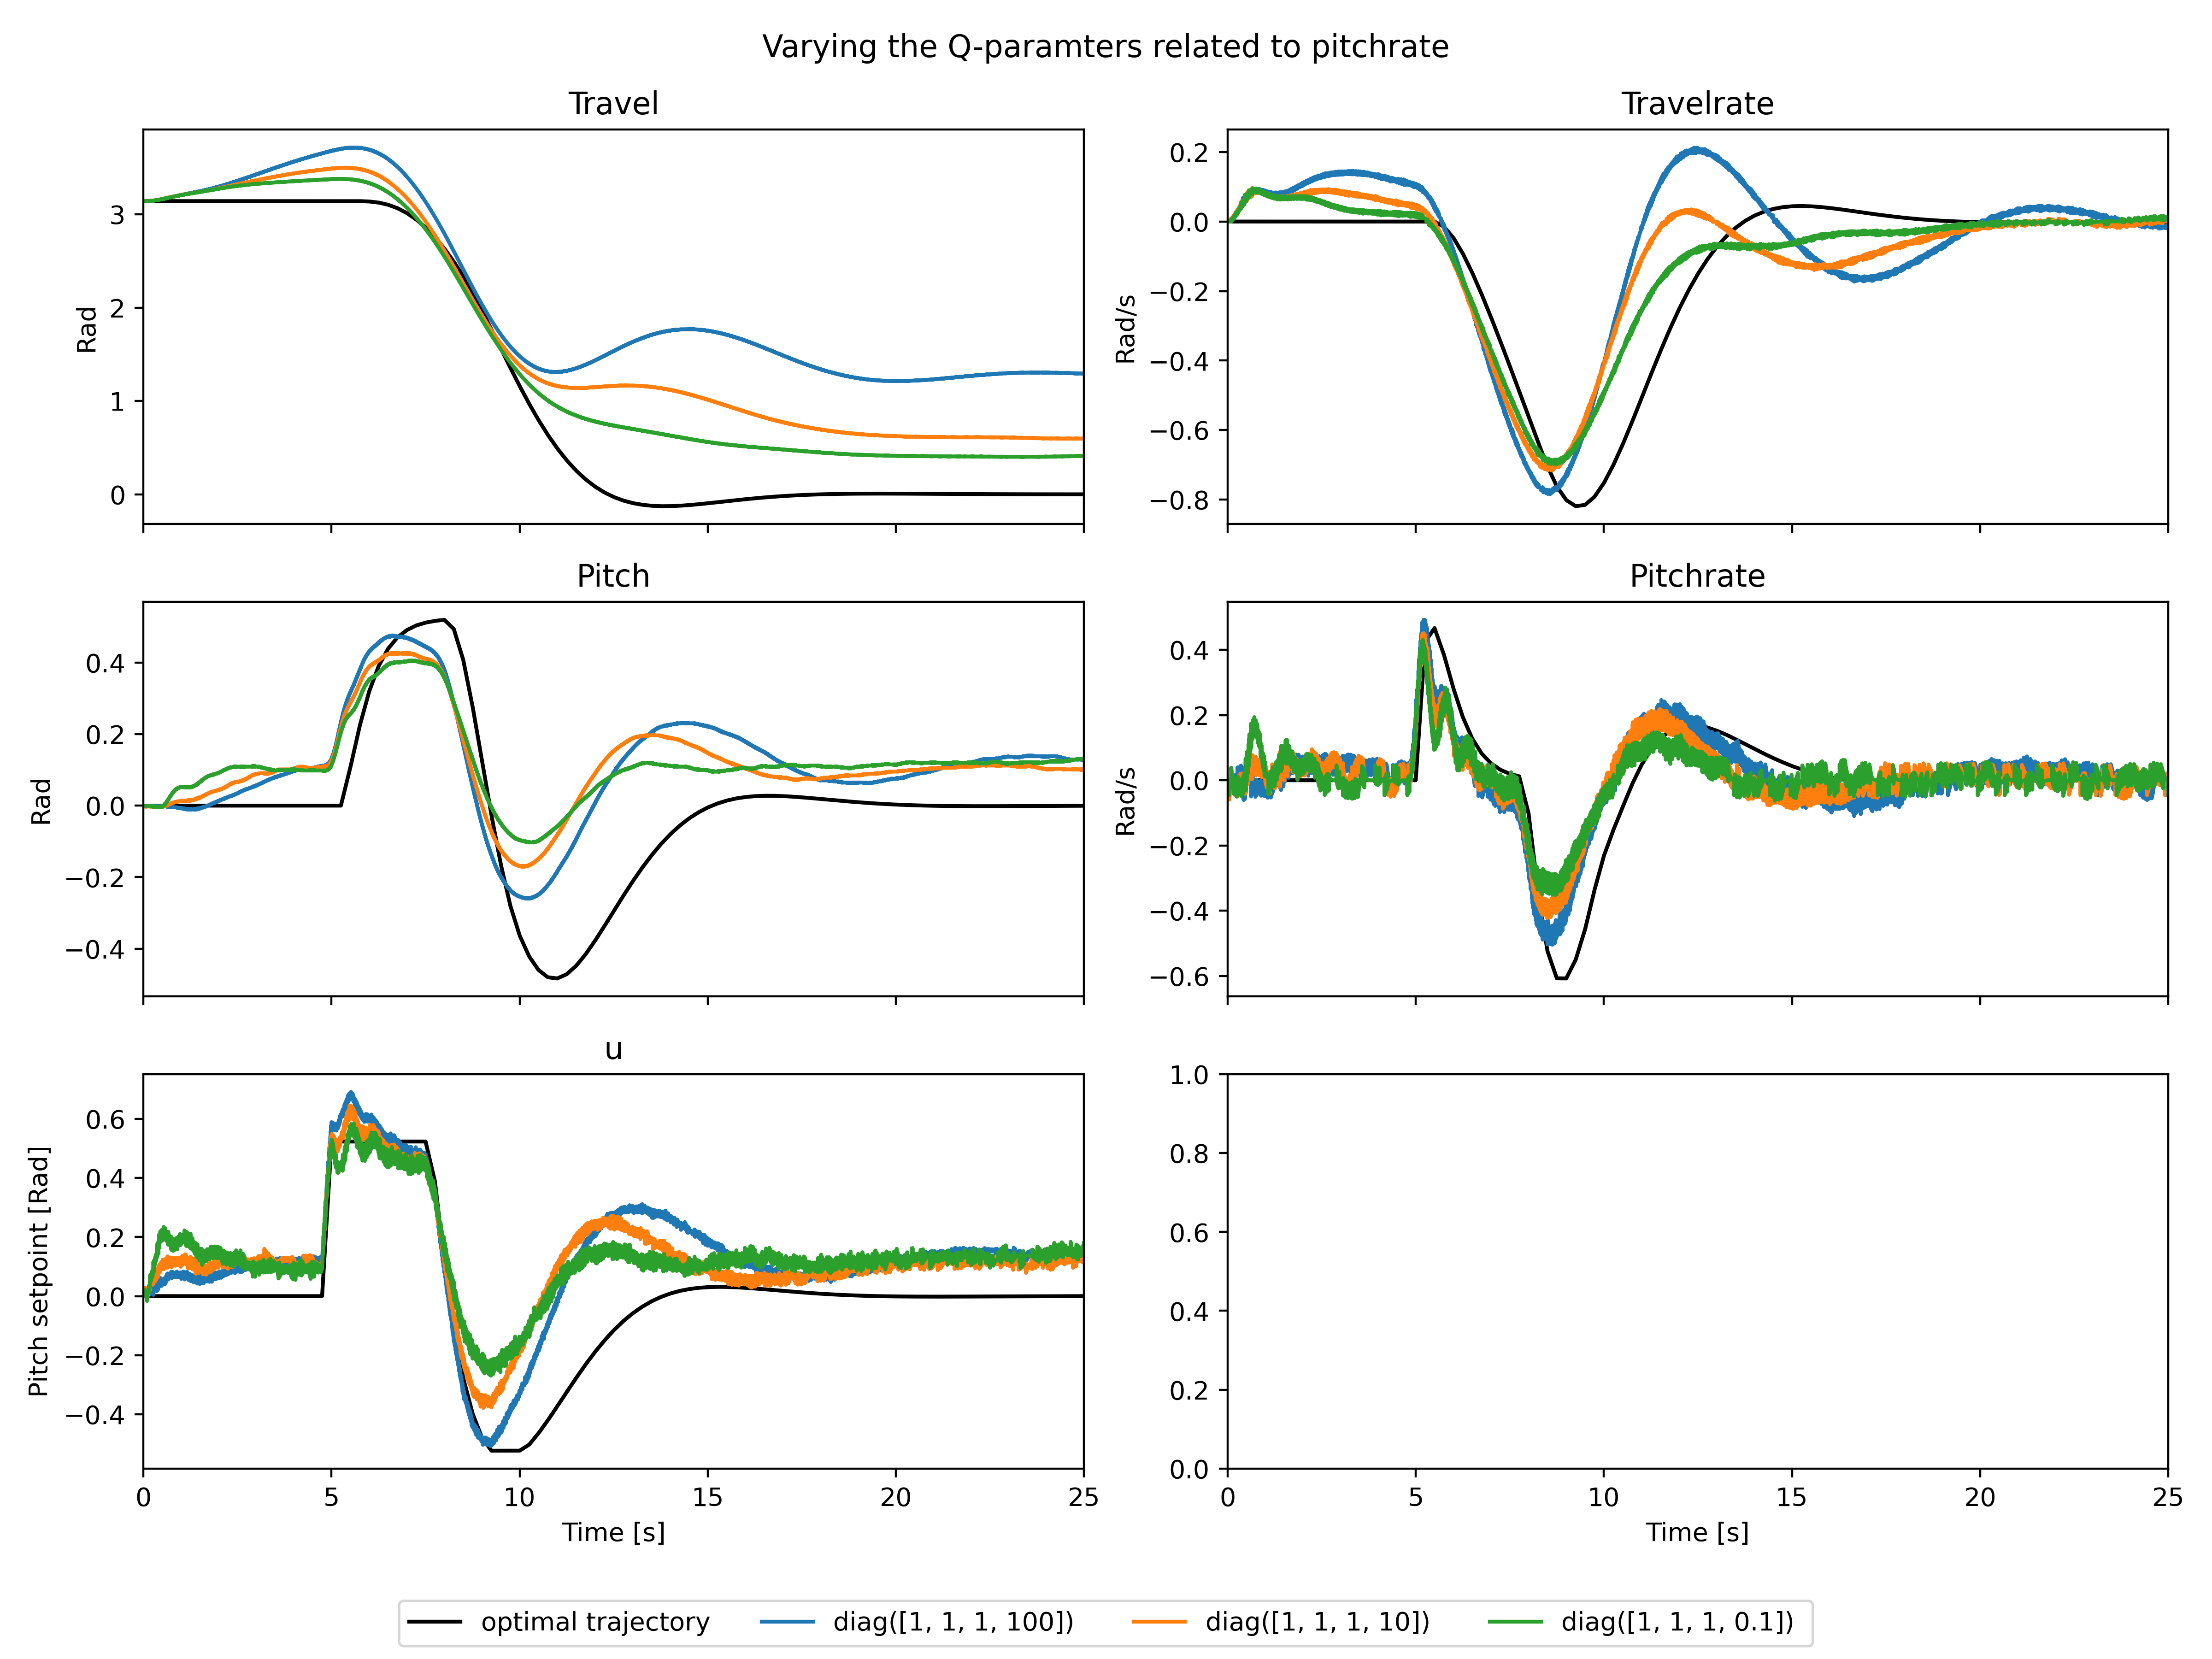
\includegraphics[width=0.8\linewidth]{figures/LAB3_Q_variations_pitchrate.png}
	\caption{Changing the weight of the pitchrate state, $R=1$. This was quite similar to \cref{fig:LAB3_Q_variations_pitch} but there is less oscillation.}
	\label{fig:LAB3_Q_variations_pitchrate}
\end{figure}
\subsubsection{Final tuning}
\todo[inline]{Oppgaven sier: ``.... Justify your choice''. Jeg tolker dette som at vi skal ha en final tuning.}
\missingfigure{Figure of final tuning}

\clearpage

\subsection{MATLAB and Simulink}
\lstinputlisting[caption= {MATLAB code for lab 3}, label={lst:lab3_matlab}]{code/problem_3.m}
\subsubsection{Simulink}
\begin{figure}[h]
	\centering
	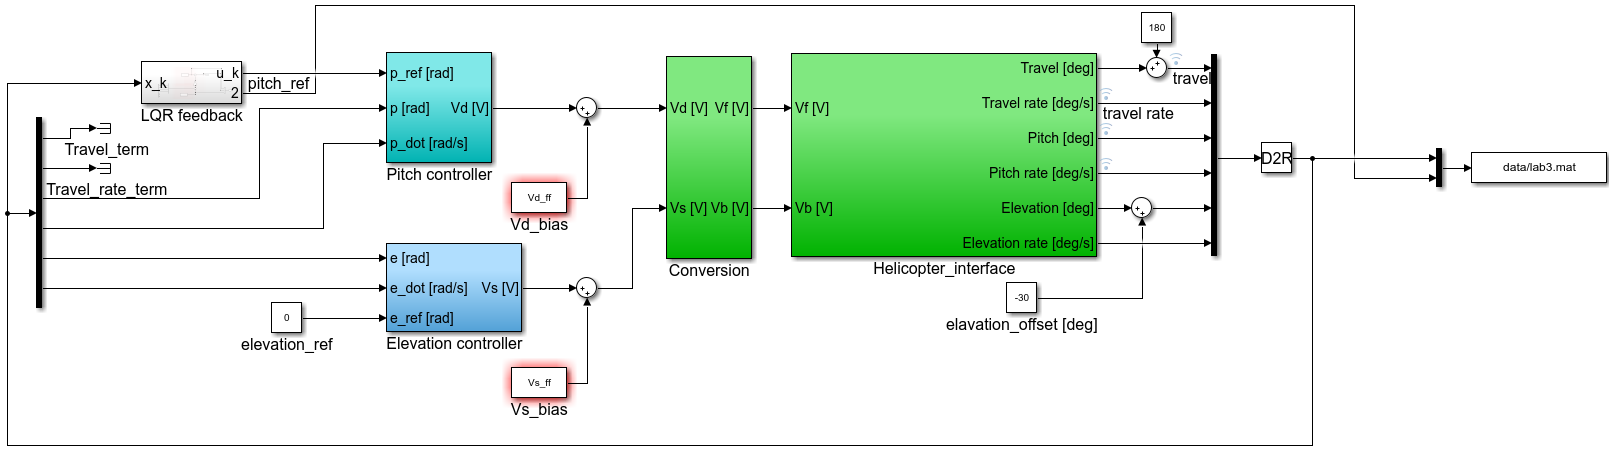
\includegraphics[width=1\linewidth, keepaspectratio]{code/lab3_simulink_1}
	\caption{Simulink diagram used in lab 3.}
	\label{fig:lab3_simulink}
\end{figure}
\begin{figure}[h]
	\centering
	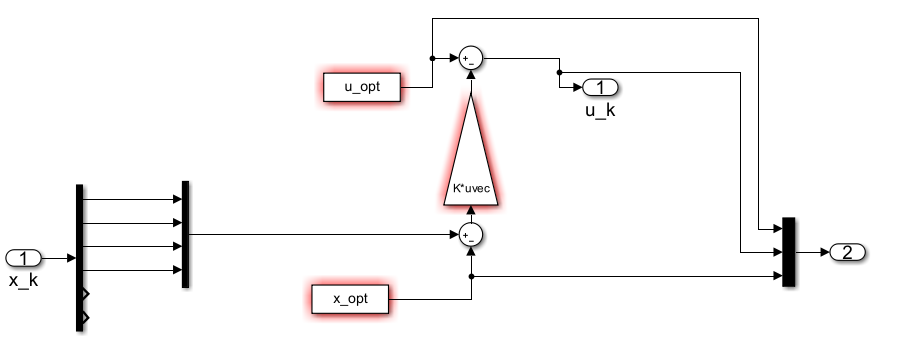
\includegraphics[width=1\linewidth, keepaspectratio]{code/lab3_simulink_2}
	\caption{``LQR Feedback'' subsystem in \cref{fig:lab3_simulink}}
	\label{fig:lab3_simulink_lqr}
\end{figure}
\end{document}